%\documentclass[a4paper, 11pt]{article}
\documentclass[UTF8]{ctexart}

\usepackage{amsmath}
\usepackage{graphicx}
\usepackage{geometry}
\usepackage{listings}
\usepackage{hyperref}
\usepackage{float} 
\usepackage{fontspec}
\setmonofont{Consolas}

\usepackage{xcolor}
\usepackage{enumerate}
\usepackage{array}
\usepackage{ulem}
\usepackage{titlesec} %自定义多级标题格式的宏包
\CTEXsetup[format={\Large\bfseries}]{section}
\CTEXsetup[format={\large\bfseries}]{subsection}

\geometry{scale=0.8}
\linespread{1.5}
\title{	
\normalfont \normalsize
\textsc{School of Computer Science, Sun Yat-sen University} \\ [25pt] %textsc small capital letters
\rule{\textwidth}{0.5pt} \\[0.4cm] % Thin top horizontal rule
\huge  E05 SAT Problem \\ % The assignment title
\rule{\textwidth}{2pt} \\[0.5cm] % Thick bottom horizontal rule
\author{19335016 HaoRan Chen}
\date{\normalsize \today} 
}

\begin{document}
\maketitle
\tableofcontents
\newpage

\section{SAT}
In logic and computer science, the Boolean satisfiability problem (SAT) is the problem of determining if there exists an interpretation that satisfies a given Boolean formula.

In other words, it asks whether the variables of a given Boolean formula can be consistently replaced by the values TRUE or FALSE in such a way that the formula evaluates to TRUE.

If this is the case, the formula is called satisfiable. On the other hand, if no such assignment exists, the function expressed by the formula is FALSE for all possible variable assignments and the formula is unsatisfiable.

\begin{figure}[!h]
    \centering
    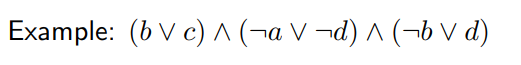
\includegraphics[width=10cm]{pic/example.png}
    \caption{SAT Problem}
    \label{fig:my_label}
\end{figure}

\section{Tasks}
\begin{enumerate}

\item  Please solve the problem in \texttt{data.txt}.

\item  Write the related codes and take a screenshot of the running results in the file named E05$\_$YourNumber.pdf, and send it to ai$\_$course2021@163.com.

\end{enumerate}

\section{Codes}
\begin{figure}[!h]
    \centering
    \includegraphics[width=0.8\textwidth]{../climb.bmp}
    \caption{爬山算法}
\end{figure}
在具体实现中, 我选择邻居的思路是贪心优先选择最优邻居, 进行递归.
\newpage
\begin{lstlisting}[language = C++, numbers=left,numberstyle=\tiny,keywordstyle=\color{blue!70},commentstyle=\color{red!50!green!50!blue!50},frame=shadowbox,rulesepcolor=\color{red!20!green!20!blue!20},basicstyle=\ttfamily]
#include <iostream>
#include <fstream>
#include <string>
#include <vector>
#include <cmath>
#include <ctime>
#include <cstdlib>
#include <algorithm>
#include <bitset>
#include <windows.h>
using namespace std;

int var_num, clause_num;
vector<vector<int> > var2clause;
vector<vector<int> > clause2var;
LARGE_INTEGER start_time, end_time, frequency;

int check_clause(vector<int>& c2v, vector<int>& var_value) {
    for (int num:c2v) {
        if ((num > 0 &&  var_value[abs(num)-1]) || 
        (num < 0 && !var_value[abs(num)-1])) {
            return 1;
        }
    }
    return 0;
}

struct State{
    vector<int> var_value;    // 变量值列表,找到一组变量赋值使得clause真值表全为1
    vector<int> clause_truth; // clause真值表
    State(){
        var_value.resize(var_num);
        clause_truth.resize(clause_num);
    }
};

bool cmp(State a, State b){
    int n1 = count(a.clause_truth.begin(), a.clause_truth.end(), 1);
    int n2 = count(b.clause_truth.begin(), b.clause_truth.end(), 1);
    return  n1 > n2;
}

vector<int> res_clause_truthfulness, res_var_value;
void serach(State *neiberState, State oriState){
    int true_num = count(oriState.clause_truth.begin(), 
    oriState.clause_truth.end(), 1);
    if(true_num == clause_num){//找到全局最优解
        QueryPerformanceCounter(&end_time);
        printf("clause_truth: \n");
        for(int _=0; _<clause_num; _++){
            printf("%d ", oriState.clause_truth[_]);
        }
        printf("\nvar_value: \n");
        for(int _=0; _<var_num; _++){
            printf("%d ", oriState.var_value[_]);
        }
        long long dur_time = (end_time.QuadPart-start_time.QuadPart)
        *1000000 / frequency.QuadPart;
        printf("Total Time is %lld us\n", dur_time);
        exit(0);
    }
    for(int i = 0; i < var_num; i++){
        int n1 = count(neiberState[i].clause_truth.begin(), 
        neiberState[i].clause_truth.end(), 1);
        int n2 = count(oriState.clause_truth.begin(), 
        oriState.clause_truth.end(), 1);
        if(n1 <= n2) break;
        State nextState[var_num];
        for(int i=0; i<var_num; i++){
            nextState[i].var_value.assign(neiberState[i].var_value.begin(), 
            neiberState[i].var_value.end());
            nextState[i].var_value[i] ^= 1;
            for(int j=0; j<clause_num; j++)
            nextState[i].clause_truth[j]=check_clause(clause2var[j], 
            nextState[i].var_value);
        }
        sort(nextState, nextState+var_num, cmp);
        serach(nextState, neiberState[i]);
    }
}

int main() {
    QueryPerformanceFrequency(&frequency);
    fstream fin; fin.open("data.txt");
    // 读取文件头
    string p, cnf; fin >> p >> cnf >> var_num >> clause_num;
    
    //printf("var_num = %d  clause_num = %d\n", var_num, clause_num);
    // 读取文件内容对两个map进行初始化
    var2clause.resize(var_num);
    clause2var.resize(clause_num);
    for (int clause_id = 0; clause_id < clause_num; clause_id++) {
        int var_id = -1;
        fin >> var_id;
        while (var_id != 0) {
            clause2var[clause_id].push_back(var_id);
            var2clause[abs(var_id)-1].push_back(clause_id);
            fin >> var_id;
        }
    }
    
    State oriState;
    for(int i = 0; i < var_num; i++) 
    oriState.var_value[i] = (rand() % 2);
    
    //for(int i=0; i < var_num; i++) 
    //    printf("%d ", oriState.var_value[i]);puts("");
    
    for(int i = 0; i < clause_num; i++) 
    oriState.clause_truth[i] = check_clause(clause2var[i], 
    oriState.var_value);
    
    //for(int i=0; i < clause_num; i++) 
    //    printf("%d ", oriState.clause_truth[i]);puts("");
    
    int num = count(oriState.clause_truth.begin(), 
    oriState.clause_truth.end(), 1);
    //printf("origin clause_truth count is %d\n", num);
    
    State neiberState[var_num];
    for(int i=0; i<var_num; i++){
        neiberState[i].var_value.assign(oriState.var_value.begin(), 
        oriState.var_value.end());
        neiberState[i].var_value[i] ^= 1;
        for(int j=0; j<clause_num; j++)
        neiberState[i].clause_truth[j]=check_clause(clause2var[j], 
        neiberState[i].var_value);
    }
    sort(neiberState, neiberState+var_num, cmp);
    //贪心优先选择最好的邻居
    
    puts("neiberState clause_truth:");
    /*
    for(int i=0; i<var_num; i++){
        int _ = count(neiberState[i].clause_truth.begin(),
        neiberState[i].clause_truth.end(), 1);
        printf("%d ", _);
    } puts("");
    */
    QueryPerformanceCounter(&start_time);
    serach(neiberState, oriState);
    
    return 0;
} 
\end{lstlisting}

\section{Results}
由于爬山算法解SAT问题性能较差, 且具有很大的随机性, 尤其是样例变量数、约束条件较多, 代码实验结果复现性较差, 在绝大多数情况下都只能得到局部最优解, 很难得到全局最优解,在多次运行之后才终于得到相对满意的结果, 故这份代码仅作参考, 并不能保证一定得到好的结果.
\begin{figure}[H]
    \centering
    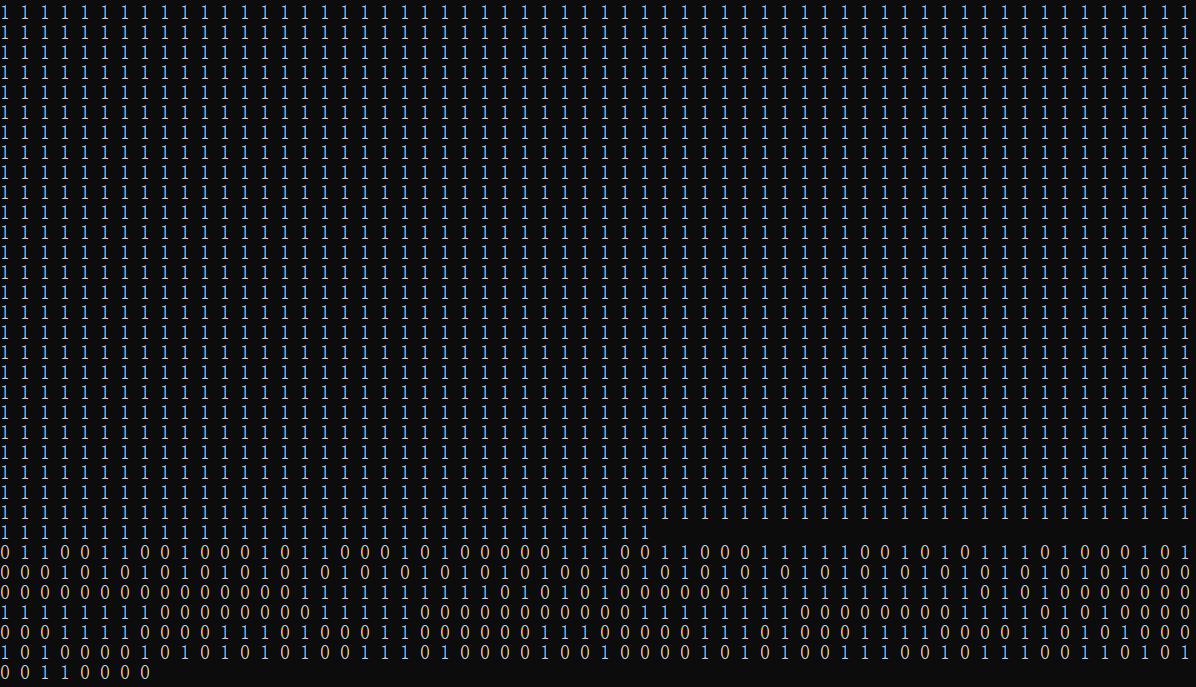
\includegraphics[width=0.8\textwidth]{res.bmp}
    \caption{实验结果}
\end{figure}


%\clearpage
%\bibliography{E:/Papers/LiuLab}
%\bibliographystyle{apalike}
\end{document} 
%%% Local Variables:
%%% mode: latex
%%% TeX-master: t
%%% End:

